\originalchapter{作业四：热量、磁体与微正则计数}
\psource{8.044，2013 春，PS4，3 月 6 日截止。中文题面；据官方答案核对的 AI 独立解答。磁功沿原课约定为 $H\dd M$。}
\originalsection{1．恒压热容}
\begin{exercise}
对简单流体证明 $C_P=(\partial U/\partial T)_P+\alpha VP$。解释为什么 $C_P$ 可比第一项小或大；提示由第一定律把热量展开成 $T,P$ 微分。
\end{exercise}
\begin{solution}
$\delta Q=\dd U+P\dd V$，恒压时除以 $\dd T$ 得所求式。$\alpha=V^{-1}(\partial V/\partial T)_P$ 可负亦可正；这与稳定性要求 $C_P\ge C_V$ 并不矛盾，因为后者比较的是另一项。
\end{solution}
\originalsection{2．三路径加热气体}
\begin{exercise}
理想气体 $C_V=5N\kb/2$，$U$ 与体积无关。从 $a=(V_1,P_1)$ 到 $b=(2V_1,2P_1)$：acb 先恒容升压后恒压膨胀，adb 先恒压膨胀后恒容升压，ab 为直线。(a) 以 $N,\kb,T_1$ 求三路输入热量；(b) 求沿 ab 的过程“热容”。
\end{exercise}
\begin{solution}
$T_b=4T_1$，$\Delta U=15N\kb T_1/2$。气体做功三路分别为 $2,1,3/2$ 倍 $P_1V_1=N\kb T_1$，故 $Q_{acb}=19N\kb T_1/2$、$Q_{adb}=17N\kb T_1/2$、$Q_{ab}=9N\kb T_1$。直线 $P=P_1V/V_1$ 给 $\dd T=2P\dd V/(N\kb)$，故 $C_{ab}=C_V+N\kb/2=3N\kb$，非状态函数的固定热容。
\end{solution}
\originalsection{3．Curie 顺磁体的热力学}
\begin{exercise}
一般简单磁体有测量量 $\chi_T=(\partial M/\partial H)_T$、$M_T=(\partial M/\partial T)_H$、$C_M,C_H$。特例 $M=aH/T$，$(\partial U/\partial M)_T=0$，$C_M=bT$，$U(0,0)=0$。
(a) 用 $T,M$ 表示 $C_M,C_H-C_M,\dd U$；(b) 对特例求 $C_H,U$；(c) 改用 $H,M$ 写一般 $\dd U$ 并比较 $\dd M$ 系数；(d) 特例消去 $T$，积分检验；(e) 求一般绝热 $(\partial T/\partial M)_{\delta Q=0}$；(f) 求经过 $T_0,M_0$ 的特例绝热线；(g) 在 $M$--$H$ 图画等温线，说明同点绝热线斜率较小。
\end{exercise}
\begin{solution}
设 $A=(\partial U/\partial M)_T$。(a) $C_M=U_T|_M$，$C_H-C_M=(A-H)M_T$，$\dd U=C_M\dd T+[H+(C_H-C_M)/M_T]\dd M$；当 $M_T=0$ 时须保留第一式而不用除式。(b) $U=bT^2/2$，$C_H=bT+aH^2/T^2=bT+M^2/a$。(c) 由 $\dd M=\chi_T\dd H+M_T\dd T$，
\[\dd U=-\frac{C_M\chi_T}{M_T}\dd H+\left(H+\frac{C_H}{M_T}\right)\dd M.\]
$\dd M$ 系数是 $U_M|_H$，不等于 $U_M|_T$。(d) $T=aH/M$ 给 $\dd U=ba^2H\dd H/M^2-ba^2H^2\dd M/M^3$，积分得 $ba^2H^2/(2M^2)=bT^2/2$。
(e) $\delta Q=\dd U-H\dd M=0$ 给 $\dd T/\dd M=(H-A)/C_M$。(f) 特例 $\dd T/\dd M=M/(ab)$，$T=T_0+(M^2-M_0^2)/(2ab)$。(g) 等温直线斜率 $a/T$，绝热斜率 $\chi_T/[1+M^2/(abT)]<\chi_T$（$a,b,T>0$）。下面取 $a=b=1,T_0=M_0=H_0=1$，绝热线用参数 $M$ 作图。
\end{solution}
\begin{center}\begin{tikzpicture}\begin{axis}[width=7cm,height=4cm,xmin=0,xmax=2,ymin=0,ymax=1.7,xlabel={$H$},ylabel={$M$},legend style={font=\small}]
\addplot[domain=0:2]{x};\addlegendentry{等温}
\addplot[domain=0:1.4,variable=\t,thick] ({t*(1+(t*t-1)/2)},{t});\addlegendentry{绝热}\end{axis}\end{tikzpicture}\end{center}
\originalsection{4．经典磁矩}
\begin{exercise}
$N$ 个固定晶格点上的独立经典磁矩，长度 $\mu$，方向可在三维旋转，$m_i=\mu_{iz}$，$M=\sum m_i$，$E=-HM$，$H>0$。
(a) 给 $m_i,M,E$ 的允许范围；(b) 指定微态需多少变量；小磁化时 $\Omega\simeq(2\mu)^N\exp[-3M^2/(2N\mu^2)]$；(c) 微正则求 $M(H,T)$；(d) 何时不物理、近似适用何温度；(e) 指定一矩 $m$ 后的 $\Omega'$ 是什么；(f) 保留 $m$ 的一次项求并画密度、验归一化；(g) 求平均比较预期。
\end{exercise}
\begin{solution}
(a) $-\mu\le m_i\le\mu$、$-N\mu\le M\le N\mu$、$-N\mu H\le E\le N\mu H$。(b) 每方向需两个角，共 $2N$ 个；能量计数中方位角的常数因子可约去。(c) $1/T=\partial S/\partial E=3\kb M/(N\mu^2H)$，故 $M=N\mu^2H/(3\kb T)$。(d) 若 $\kb T<\mu H/3$ 会超过饱和范围；可靠近似要求更强的 $\mu H/(\kb T)\ll1$。(e) $\Omega'=\Omega_{N-1}(M-m)$。(f) 大 $N$ 展开归一化后 $p(m)\simeq[1+3Mm/(N\mu^2)]/(2\mu)$，$|m|\le\mu$，是略向正端倾斜的直线；奇项积分零。(g) $\avg m=M/N=\mu^2H/(3\kb T)$，符合总磁化。该线性近似只在小偏置时保持非负。
\end{solution}
\begin{center}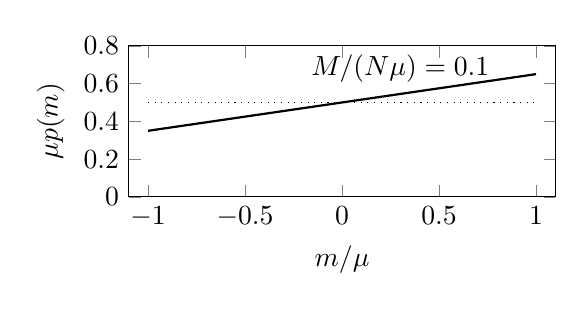
\begin{tikzpicture}\begin{axis}[width=7cm,height=3.5cm,xmin=-1.1,xmax=1.1,ymin=0,ymax=.8,xlabel={$m/\mu$},ylabel={$\mu p(m)$}]\addplot[domain=-1:1,thick]{.5*(1+.3*x)};\addplot[domain=-1:1,dotted]{.5};\node at(axis cs:.3,.68){$M/(N\mu)=0.1$};\end{axis}\end{tikzpicture}\end{center}
\originalsection{5．熵弹性链}
\begin{exercise}
$N$ 个长度 $l$ 的链元可向左或右，弯折不耗能；$N=n_++n_-$，$L=l(n_+-n_-)$。(a) 求 $S(N,n_+)$；(b) 求张力 $F(T,N,n_+)$；(c) 反解 $L(N,T,F)$；(d) 用高温极限求恒张力热膨胀系数，并预测负重橡皮筋受热时重物升降。
\end{exercise}
\begin{solution}
(a) $S=\kb\ln[N!/(n_+!n_-!)]$；大 $N$ 用 Stirling。(b) $\dd U=T\dd S+F\dd L=0$ 给 $F=-T S_L=\kb T\ln(n_+/n_-)/(2l)$。(c) $L=Nl\tanh(Fl/(\kb T))$。(d) 高温/弱拉伸 $L\simeq NFl^2/(\kb T)$，$\alpha=-1/T$；受热缩短，重物上升。理想链忽略真实链元长度的温度变化。
\end{solution}
\originalsection{6．经典谐振子的微正则系综}
\begin{exercise}
$N$ 个相同谐振子有微弱非零耦合，总能 $\sum_i[p_i^2/(2m)+m\omega^2q_i^2/2]=E$。
(a) 变换 $x_i=p_i/\sqrt{2m}$、$x_{N+i}=q_i\sqrt{m\omega^2/2}$，求 $2N$ 维球体积及原相空间体积 $\Phi(E)$；(b) 求熵；(c) 求温度与能量；(d) 求一振子 $p(p_i,q_i)$ 并画形状。
\end{exercise}
\begin{solution}
(a) 半径 $\sqrt E$ 球体积 $\pi^NE^N/N!$；每一对 Jacobian $2/\omega$，所以 $\Phi=(2\pi E/\omega)^N/N!$。以每对 $h$ 为态单元，计数为 $(E/\hbar\omega)^N/N!$。(b) 体积熵为 $S_G=\kb[N\ln(E/\hbar\omega)-\ln N!]$；能壳熵 $S_B=\kb\ln[(E/\hbar\omega)^{N-1}\Delta E/((N-1)!\hbar\omega)]$，两者有限 $N$ 不同。(c) 前者 $E=N\kb T$，后者 $E=(N-1)\kb T$；热力学极限一致。(d) 对能壳边缘，$N>1$，
\[p(p,q)=\frac{(N-1)\omega}{2\pi E}\left(1-\frac{\epsilon(p,q)}E\right)^{N-2},\quad0\le\epsilon\le E.\]
大 $N$ 为 $\omega e^{-\epsilon/(\kb T)}/(2\pi\kb T)$，中心峰、等密度线为椭圆，$q,p$ 各高斯。单振子能量密度为 $(N-1)E^{-1}(1-\epsilon/E)^{N-2}$；沿椭圆积分即归一化。
\end{solution}
\begin{center}\begin{tikzpicture}[x=1.1cm,y=.7cm]\draw[->](-2.5,0)--(2.5,0)node[right]{$q$};\draw[->](0,-2.5)--(0,2.5)node[above]{$p$};\foreach \r in {.6,1.2,1.8}{\draw (0,0)ellipse[x radius=\r,y radius=\r];}\node at(1.5,2.3){中心密度最高};\end{tikzpicture}\end{center}
